% Options for packages loaded elsewhere
\PassOptionsToPackage{unicode}{hyperref}
\PassOptionsToPackage{hyphens}{url}
%
\documentclass[
]{article}
\usepackage{amsmath,amssymb}
\usepackage{lmodern}
\usepackage{iftex}
\ifPDFTeX
  \usepackage[T1]{fontenc}
  \usepackage[utf8]{inputenc}
  \usepackage{textcomp} % provide euro and other symbols
\else % if luatex or xetex
  \usepackage{unicode-math}
  \defaultfontfeatures{Scale=MatchLowercase}
  \defaultfontfeatures[\rmfamily]{Ligatures=TeX,Scale=1}
\fi
% Use upquote if available, for straight quotes in verbatim environments
\IfFileExists{upquote.sty}{\usepackage{upquote}}{}
\IfFileExists{microtype.sty}{% use microtype if available
  \usepackage[]{microtype}
  \UseMicrotypeSet[protrusion]{basicmath} % disable protrusion for tt fonts
}{}
\makeatletter
\@ifundefined{KOMAClassName}{% if non-KOMA class
  \IfFileExists{parskip.sty}{%
    \usepackage{parskip}
  }{% else
    \setlength{\parindent}{0pt}
    \setlength{\parskip}{6pt plus 2pt minus 1pt}}
}{% if KOMA class
  \KOMAoptions{parskip=half}}
\makeatother
\usepackage{xcolor}
\usepackage[margin=1in]{geometry}
\usepackage{color}
\usepackage{fancyvrb}
\newcommand{\VerbBar}{|}
\newcommand{\VERB}{\Verb[commandchars=\\\{\}]}
\DefineVerbatimEnvironment{Highlighting}{Verbatim}{commandchars=\\\{\}}
% Add ',fontsize=\small' for more characters per line
\usepackage{framed}
\definecolor{shadecolor}{RGB}{248,248,248}
\newenvironment{Shaded}{\begin{snugshade}}{\end{snugshade}}
\newcommand{\AlertTok}[1]{\textcolor[rgb]{0.94,0.16,0.16}{#1}}
\newcommand{\AnnotationTok}[1]{\textcolor[rgb]{0.56,0.35,0.01}{\textbf{\textit{#1}}}}
\newcommand{\AttributeTok}[1]{\textcolor[rgb]{0.77,0.63,0.00}{#1}}
\newcommand{\BaseNTok}[1]{\textcolor[rgb]{0.00,0.00,0.81}{#1}}
\newcommand{\BuiltInTok}[1]{#1}
\newcommand{\CharTok}[1]{\textcolor[rgb]{0.31,0.60,0.02}{#1}}
\newcommand{\CommentTok}[1]{\textcolor[rgb]{0.56,0.35,0.01}{\textit{#1}}}
\newcommand{\CommentVarTok}[1]{\textcolor[rgb]{0.56,0.35,0.01}{\textbf{\textit{#1}}}}
\newcommand{\ConstantTok}[1]{\textcolor[rgb]{0.00,0.00,0.00}{#1}}
\newcommand{\ControlFlowTok}[1]{\textcolor[rgb]{0.13,0.29,0.53}{\textbf{#1}}}
\newcommand{\DataTypeTok}[1]{\textcolor[rgb]{0.13,0.29,0.53}{#1}}
\newcommand{\DecValTok}[1]{\textcolor[rgb]{0.00,0.00,0.81}{#1}}
\newcommand{\DocumentationTok}[1]{\textcolor[rgb]{0.56,0.35,0.01}{\textbf{\textit{#1}}}}
\newcommand{\ErrorTok}[1]{\textcolor[rgb]{0.64,0.00,0.00}{\textbf{#1}}}
\newcommand{\ExtensionTok}[1]{#1}
\newcommand{\FloatTok}[1]{\textcolor[rgb]{0.00,0.00,0.81}{#1}}
\newcommand{\FunctionTok}[1]{\textcolor[rgb]{0.00,0.00,0.00}{#1}}
\newcommand{\ImportTok}[1]{#1}
\newcommand{\InformationTok}[1]{\textcolor[rgb]{0.56,0.35,0.01}{\textbf{\textit{#1}}}}
\newcommand{\KeywordTok}[1]{\textcolor[rgb]{0.13,0.29,0.53}{\textbf{#1}}}
\newcommand{\NormalTok}[1]{#1}
\newcommand{\OperatorTok}[1]{\textcolor[rgb]{0.81,0.36,0.00}{\textbf{#1}}}
\newcommand{\OtherTok}[1]{\textcolor[rgb]{0.56,0.35,0.01}{#1}}
\newcommand{\PreprocessorTok}[1]{\textcolor[rgb]{0.56,0.35,0.01}{\textit{#1}}}
\newcommand{\RegionMarkerTok}[1]{#1}
\newcommand{\SpecialCharTok}[1]{\textcolor[rgb]{0.00,0.00,0.00}{#1}}
\newcommand{\SpecialStringTok}[1]{\textcolor[rgb]{0.31,0.60,0.02}{#1}}
\newcommand{\StringTok}[1]{\textcolor[rgb]{0.31,0.60,0.02}{#1}}
\newcommand{\VariableTok}[1]{\textcolor[rgb]{0.00,0.00,0.00}{#1}}
\newcommand{\VerbatimStringTok}[1]{\textcolor[rgb]{0.31,0.60,0.02}{#1}}
\newcommand{\WarningTok}[1]{\textcolor[rgb]{0.56,0.35,0.01}{\textbf{\textit{#1}}}}
\usepackage{graphicx}
\makeatletter
\def\maxwidth{\ifdim\Gin@nat@width>\linewidth\linewidth\else\Gin@nat@width\fi}
\def\maxheight{\ifdim\Gin@nat@height>\textheight\textheight\else\Gin@nat@height\fi}
\makeatother
% Scale images if necessary, so that they will not overflow the page
% margins by default, and it is still possible to overwrite the defaults
% using explicit options in \includegraphics[width, height, ...]{}
\setkeys{Gin}{width=\maxwidth,height=\maxheight,keepaspectratio}
% Set default figure placement to htbp
\makeatletter
\def\fps@figure{htbp}
\makeatother
\setlength{\emergencystretch}{3em} % prevent overfull lines
\providecommand{\tightlist}{%
  \setlength{\itemsep}{0pt}\setlength{\parskip}{0pt}}
\setcounter{secnumdepth}{-\maxdimen} % remove section numbering
\usepackage{booktabs}
\usepackage{longtable}
\usepackage{array}
\usepackage{multirow}
\usepackage{wrapfig}
\usepackage{float}
\usepackage{colortbl}
\usepackage{pdflscape}
\usepackage{tabu}
\usepackage{threeparttable}
\usepackage{threeparttablex}
\usepackage[normalem]{ulem}
\usepackage{makecell}
\usepackage{xcolor}
\ifLuaTeX
  \usepackage{selnolig}  % disable illegal ligatures
\fi
\IfFileExists{bookmark.sty}{\usepackage{bookmark}}{\usepackage{hyperref}}
\IfFileExists{xurl.sty}{\usepackage{xurl}}{} % add URL line breaks if available
\urlstyle{same} % disable monospaced font for URLs
\hypersetup{
  pdftitle={Práctica 6},
  pdfauthor={Carlos Mota Romero},
  hidelinks,
  pdfcreator={LaTeX via pandoc}}

\title{Práctica 6}
\author{Carlos Mota Romero}
\date{2023-03-27}

\begin{document}
\maketitle

\hypertarget{ejercicio-1-instalaciuxf3n-de-paquetes}{%
\subsection{Ejercicio 1: Instalación de
paquetes}\label{ejercicio-1-instalaciuxf3n-de-paquetes}}

Para instalar diversas librerías que necesitaremos para trabajar en el
siguiente ejercicio, usaremos el comando \texttt{install.packages} y
para activarlos lo haremos con el comando \texttt{library}

\begin{Shaded}
\begin{Highlighting}[]
\FunctionTok{install.packages}\NormalTok{(}\StringTok{"MASS"}\NormalTok{, }\AttributeTok{repos =} \StringTok{"http://cran.us.r{-}project.org"}\NormalTok{)}
\end{Highlighting}
\end{Shaded}

\begin{verbatim}
## Installing package into 'C:/Users/Lacros/AppData/Local/R/win-library/4.2'
## (as 'lib' is unspecified)
\end{verbatim}

\begin{verbatim}
## package 'MASS' successfully unpacked and MD5 sums checked
\end{verbatim}

\begin{verbatim}
## Warning: cannot remove prior installation of package 'MASS'
\end{verbatim}

\begin{verbatim}
## Warning in file.copy(savedcopy, lib, recursive = TRUE): problema al copiar
## C:\Users\Lacros\AppData\Local\R\win-library\4.2\00LOCK\MASS\libs\x64\MASS.dll a
## C:\Users\Lacros\AppData\Local\R\win-library\4.2\MASS\libs\x64\MASS.dll:
## Permission denied
\end{verbatim}

\begin{verbatim}
## Warning: restored 'MASS'
\end{verbatim}

\begin{verbatim}
## 
## The downloaded binary packages are in
##  C:\Users\Lacros\AppData\Local\Temp\RtmpaAmadV\downloaded_packages
\end{verbatim}

\begin{Shaded}
\begin{Highlighting}[]
\FunctionTok{library}\NormalTok{(MASS)}
\end{Highlighting}
\end{Shaded}

\begin{verbatim}
## Warning: package 'MASS' was built under R version 4.2.3
\end{verbatim}

\begin{Shaded}
\begin{Highlighting}[]
\FunctionTok{install.packages}\NormalTok{(}\StringTok{"caret"}\NormalTok{, }\AttributeTok{repos =} \StringTok{"http://cran.us.r{-}project.org"}\NormalTok{)}
\end{Highlighting}
\end{Shaded}

\begin{verbatim}
## Installing package into 'C:/Users/Lacros/AppData/Local/R/win-library/4.2'
## (as 'lib' is unspecified)
\end{verbatim}

\begin{verbatim}
## package 'caret' successfully unpacked and MD5 sums checked
\end{verbatim}

\begin{verbatim}
## Warning: cannot remove prior installation of package 'caret'
\end{verbatim}

\begin{verbatim}
## Warning in file.copy(savedcopy, lib, recursive = TRUE): problema al copiar
## C:\Users\Lacros\AppData\Local\R\win-library\4.2\00LOCK\caret\libs\x64\caret.dll
## a C:\Users\Lacros\AppData\Local\R\win-library\4.2\caret\libs\x64\caret.dll:
## Permission denied
\end{verbatim}

\begin{verbatim}
## Warning: restored 'caret'
\end{verbatim}

\begin{verbatim}
## 
## The downloaded binary packages are in
##  C:\Users\Lacros\AppData\Local\Temp\RtmpaAmadV\downloaded_packages
\end{verbatim}

\begin{Shaded}
\begin{Highlighting}[]
\FunctionTok{library}\NormalTok{(caret)}
\end{Highlighting}
\end{Shaded}

\begin{verbatim}
## Warning: package 'caret' was built under R version 4.2.3
\end{verbatim}

\begin{verbatim}
## Loading required package: ggplot2
\end{verbatim}

\begin{verbatim}
## Loading required package: lattice
\end{verbatim}

\begin{Shaded}
\begin{Highlighting}[]
\FunctionTok{installed.packages}\NormalTok{(}\StringTok{"stats"}\NormalTok{, }\AttributeTok{repos =} \StringTok{"http://cran.us.r{-}project.org"}\NormalTok{)}
\end{Highlighting}
\end{Shaded}

\begin{verbatim}
##      Package LibPath Version Priority Depends Imports LinkingTo Suggests
##      Enhances License License_is_FOSS License_restricts_use OS_type Archs
##      MD5sum NeedsCompilation Built
\end{verbatim}

\begin{Shaded}
\begin{Highlighting}[]
\FunctionTok{library}\NormalTok{(stats)}
\FunctionTok{install.packages}\NormalTok{(}\StringTok{"olsrr"}\NormalTok{, }\AttributeTok{repos =} \StringTok{"http://cran.us.r{-}project.org"}\NormalTok{)}
\end{Highlighting}
\end{Shaded}

\begin{verbatim}
## Installing package into 'C:/Users/Lacros/AppData/Local/R/win-library/4.2'
## (as 'lib' is unspecified)
\end{verbatim}

\begin{verbatim}
## package 'olsrr' successfully unpacked and MD5 sums checked
## 
## The downloaded binary packages are in
##  C:\Users\Lacros\AppData\Local\Temp\RtmpaAmadV\downloaded_packages
\end{verbatim}

\begin{Shaded}
\begin{Highlighting}[]
\FunctionTok{library}\NormalTok{(olsrr)}
\end{Highlighting}
\end{Shaded}

\begin{verbatim}
## Warning: package 'olsrr' was built under R version 4.2.3
\end{verbatim}

\begin{verbatim}
## 
## Attaching package: 'olsrr'
\end{verbatim}

\begin{verbatim}
## The following object is masked from 'package:MASS':
## 
##     cement
\end{verbatim}

\begin{verbatim}
## The following object is masked from 'package:datasets':
## 
##     rivers
\end{verbatim}

\begin{Shaded}
\begin{Highlighting}[]
\FunctionTok{install.packages}\NormalTok{(}\StringTok{"kableExtra"}\NormalTok{, }\AttributeTok{repos =} \StringTok{"http://cran.us.r{-}project.org"}\NormalTok{)}
\end{Highlighting}
\end{Shaded}

\begin{verbatim}
## Installing package into 'C:/Users/Lacros/AppData/Local/R/win-library/4.2'
## (as 'lib' is unspecified)
\end{verbatim}

\begin{verbatim}
## package 'kableExtra' successfully unpacked and MD5 sums checked
## 
## The downloaded binary packages are in
##  C:\Users\Lacros\AppData\Local\Temp\RtmpaAmadV\downloaded_packages
\end{verbatim}

\begin{Shaded}
\begin{Highlighting}[]
\FunctionTok{library}\NormalTok{(kableExtra)}
\end{Highlighting}
\end{Shaded}

\begin{verbatim}
## Warning: package 'kableExtra' was built under R version 4.2.3
\end{verbatim}

\begin{verbatim}
## Warning in !is.null(rmarkdown::metadata$output) && rmarkdown::metadata$output
## %in% : 'length(x) = 2 > 1' in coercion to 'logical(1)'
\end{verbatim}

\begin{Shaded}
\begin{Highlighting}[]
\FunctionTok{install.packages}\NormalTok{(}\StringTok{"knitr"}\NormalTok{, }\AttributeTok{repos =} \StringTok{"http://cran.us.r{-}project.org"}\NormalTok{)}
\end{Highlighting}
\end{Shaded}

\begin{verbatim}
## Installing package into 'C:/Users/Lacros/AppData/Local/R/win-library/4.2'
## (as 'lib' is unspecified)
\end{verbatim}

\begin{verbatim}
## package 'knitr' successfully unpacked and MD5 sums checked
## 
## The downloaded binary packages are in
##  C:\Users\Lacros\AppData\Local\Temp\RtmpaAmadV\downloaded_packages
\end{verbatim}

\begin{Shaded}
\begin{Highlighting}[]
\FunctionTok{library}\NormalTok{(knitr)}
\end{Highlighting}
\end{Shaded}

\begin{verbatim}
## Warning: package 'knitr' was built under R version 4.2.3
\end{verbatim}

\begin{Shaded}
\begin{Highlighting}[]
\FunctionTok{install.packages}\NormalTok{(}\StringTok{"rmarkdown"}\NormalTok{, }\AttributeTok{repos =} \StringTok{"http://cran.us.r{-}project.org"}\NormalTok{)}
\end{Highlighting}
\end{Shaded}

\begin{verbatim}
## Installing package into 'C:/Users/Lacros/AppData/Local/R/win-library/4.2'
## (as 'lib' is unspecified)
\end{verbatim}

\begin{verbatim}
## package 'rmarkdown' successfully unpacked and MD5 sums checked
## 
## The downloaded binary packages are in
##  C:\Users\Lacros\AppData\Local\Temp\RtmpaAmadV\downloaded_packages
\end{verbatim}

\begin{Shaded}
\begin{Highlighting}[]
\FunctionTok{library}\NormalTok{(rmarkdown)}
\end{Highlighting}
\end{Shaded}

\begin{verbatim}
## Warning: package 'rmarkdown' was built under R version 4.2.3
\end{verbatim}

\hypertarget{ejercicio-2-crear-vectores}{%
\subsection{Ejercicio 2: Crear
vectores}\label{ejercicio-2-crear-vectores}}

Creamos vectores con \texttt{c}y dotándolos de un nombre

\begin{Shaded}
\begin{Highlighting}[]
\NormalTok{y\_cuentas }\OtherTok{\textless{}{-}} \FunctionTok{c}\NormalTok{(}\DecValTok{110}\NormalTok{,}\DecValTok{2}\NormalTok{,}\DecValTok{6}\NormalTok{,}\DecValTok{98}\NormalTok{,}\DecValTok{40}\NormalTok{,}\DecValTok{94}\NormalTok{,}\DecValTok{31}\NormalTok{,}\DecValTok{5}\NormalTok{,}\DecValTok{8}\NormalTok{,}\DecValTok{10}\NormalTok{)}
\NormalTok{y\_cuentas}
\end{Highlighting}
\end{Shaded}

\begin{verbatim}
##  [1] 110   2   6  98  40  94  31   5   8  10
\end{verbatim}

\begin{Shaded}
\begin{Highlighting}[]
\NormalTok{x\_distancias }\OtherTok{\textless{}{-}} \FunctionTok{c}\NormalTok{(}\FloatTok{1.1}\NormalTok{,}\FloatTok{100.2}\NormalTok{,}\FloatTok{90.3}\NormalTok{,}\FloatTok{5.4}\NormalTok{,}\FloatTok{57.5}\NormalTok{,}\FloatTok{6.6}\NormalTok{,}\FloatTok{34.7}\NormalTok{,}\FloatTok{65.8}\NormalTok{,}\FloatTok{57.9}\NormalTok{,}\FloatTok{86.1}\NormalTok{)}
\NormalTok{x\_distancias}
\end{Highlighting}
\end{Shaded}

\begin{verbatim}
##  [1]   1.1 100.2  90.3   5.4  57.5   6.6  34.7  65.8  57.9  86.1
\end{verbatim}

\hypertarget{ejercicio-3-comprobar-la-linealidad}{%
\subsection{Ejercicio 3: Comprobar la
linealidad}\label{ejercicio-3-comprobar-la-linealidad}}

Comprobamos la linealidad de forma matemática con los comandos
\texttt{cor}y \texttt{cor.test}El primero nos da un valor que nos
informa sobre la correlacion de las variables, y el segundo nos aporta
este mismo dato con un p-value que nos informa sobre las posibilidades
de que ese valor no se deba al azar.

\begin{Shaded}
\begin{Highlighting}[]
\FunctionTok{cor}\NormalTok{(x\_distancias, y\_cuentas)}
\end{Highlighting}
\end{Shaded}

\begin{verbatim}
## [1] -0.9249824
\end{verbatim}

\begin{Shaded}
\begin{Highlighting}[]
\FunctionTok{cor.test}\NormalTok{(x\_distancias, y\_cuentas)}
\end{Highlighting}
\end{Shaded}

\begin{verbatim}
## 
##  Pearson's product-moment correlation
## 
## data:  x_distancias and y_cuentas
## t = -6.8847, df = 8, p-value = 0.0001265
## alternative hypothesis: true correlation is not equal to 0
## 95 percent confidence interval:
##  -0.9824414 -0.7072588
## sample estimates:
##        cor 
## -0.9249824
\end{verbatim}

Con esto podemos llegar a saber que mantienen una correlación inversa,
es decir que a más alejado del punto 0 menos cuentas aparecen. También
podemos saber que es una correlación fiable porque el p-value es menor a
0.05 que es lo mínimo teniendo una confianza del 95\%.

\begin{Shaded}
\begin{Highlighting}[]
\FunctionTok{plot}\NormalTok{(x\_distancias, y\_cuentas)}
\end{Highlighting}
\end{Shaded}

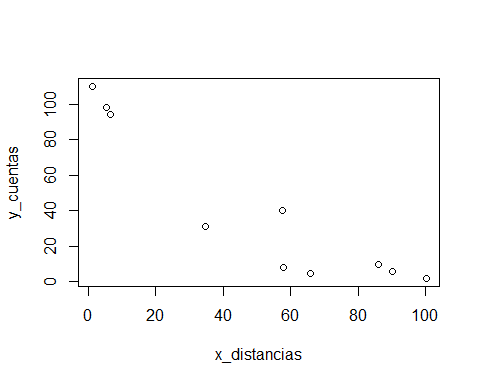
\includegraphics{Practica_6_files/figure-latex/unnamed-chunk-4-1.pdf} Al
generar en un gráfico estas dos variables podemos ver que se mantienen
gráficamente lo que habíamos asumido matemáticamente.

\hypertarget{ejercicio-4-comprobar-la-normalidad}{%
\subsection{Ejercicio 4: Comprobar la
normalidad:}\label{ejercicio-4-comprobar-la-normalidad}}

Para comprobar la normalidad de la variable explicativa (en este caso el
vector \texttt{x\_distancias}) podemos hacer un histograma (con la
función \texttt{hist}y añadiendo una linea de densidad con
\texttt{lines(density(x))}para comprobar la distribución de los valores.
Si tuviera una distribución en forma de campana, sería una variable
normal, como no es así, comprobamos que la variable explicativa no tenga
una distribución normal de los datos.

\begin{Shaded}
\begin{Highlighting}[]
\FunctionTok{hist}\NormalTok{(x\_distancias, }\AttributeTok{prob=}\ConstantTok{TRUE}\NormalTok{)}
\FunctionTok{lines}\NormalTok{(}\FunctionTok{density}\NormalTok{(x\_distancias))}
\end{Highlighting}
\end{Shaded}

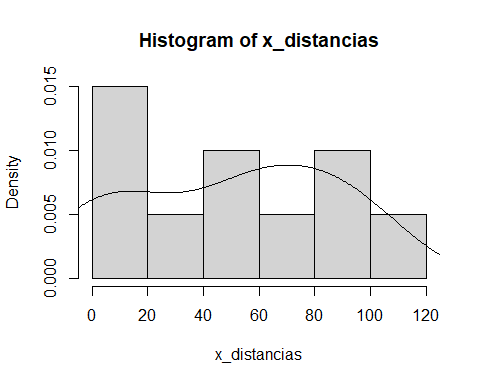
\includegraphics{Practica_6_files/figure-latex/unnamed-chunk-5-1.pdf}
Para comprobar matemáticamente y de forma automática si la distribución
de datos de una variable es normal, podemos usar la función
\texttt{shapiro.test}. Pero al tener tan pocos valores en nuestra
variable, esta función no nos da un resultado fiable. De hecho en este
caso, nos da un valor p mayor a 0'05, lo que indicaría una distribución
normal de los datos, cuando sabemos que esto no es el caso para nuestra
muestra.

\begin{Shaded}
\begin{Highlighting}[]
\FunctionTok{shapiro.test}\NormalTok{(x\_distancias)}
\end{Highlighting}
\end{Shaded}

\begin{verbatim}
## 
##  Shapiro-Wilk normality test
## 
## data:  x_distancias
## W = 0.90687, p-value = 0.2602
\end{verbatim}

\hypertarget{ejercicio-5-multiplicar-las-variables}{%
\subsection{Ejercicio 5: Multiplicar las
variables}\label{ejercicio-5-multiplicar-las-variables}}

Para multiplicar las variables utilizamos el caracter \texttt{*} y
llamamos al objeto creado con un nuevo nombre con el símbolo
\texttt{\textless{}-}.

\begin{Shaded}
\begin{Highlighting}[]
\NormalTok{xy }\OtherTok{\textless{}{-}}\NormalTok{ x\_distancias}\SpecialCharTok{*}\NormalTok{y\_cuentas}
\NormalTok{xy}
\end{Highlighting}
\end{Shaded}

\begin{verbatim}
##  [1]  121.0  200.4  541.8  529.2 2300.0  620.4 1075.7  329.0  463.2  861.0
\end{verbatim}

\#Ejercicio 6: Elevar al cuadrado Para elevar al cuadrado nuestra
variable explicativa \texttt{x\_distancias} utilizamos el símbolo
\texttt{\^{}}.

\begin{Shaded}
\begin{Highlighting}[]
\NormalTok{x\_cuadrado }\OtherTok{\textless{}{-}}\NormalTok{ x\_distancias}\SpecialCharTok{\^{}}\DecValTok{2}
\NormalTok{x\_cuadrado}
\end{Highlighting}
\end{Shaded}

\begin{verbatim}
##  [1]     1.21 10040.04  8154.09    29.16  3306.25    43.56  1204.09  4329.64
##  [9]  3352.41  7413.21
\end{verbatim}

\hypertarget{ejercicio-7-crear-un-dataframe}{%
\subsection{Ejercicio 7: Crear un
dataframe}\label{ejercicio-7-crear-un-dataframe}}

Para crear un dataframe con todos los vectores que hemos estado creando
hasta ahora, usamos la función \texttt{data.frame}.

\begin{Shaded}
\begin{Highlighting}[]
\NormalTok{tabla\_datos }\OtherTok{\textless{}{-}} \FunctionTok{data.frame}\NormalTok{(y\_cuentas, x\_distancias, xy, x\_cuadrado)}
\NormalTok{tabla\_datos}
\end{Highlighting}
\end{Shaded}

\begin{verbatim}
##    y_cuentas x_distancias     xy x_cuadrado
## 1        110          1.1  121.0       1.21
## 2          2        100.2  200.4   10040.04
## 3          6         90.3  541.8    8154.09
## 4         98          5.4  529.2      29.16
## 5         40         57.5 2300.0    3306.25
## 6         94          6.6  620.4      43.56
## 7         31         34.7 1075.7    1204.09
## 8          5         65.8  329.0    4329.64
## 9          8         57.9  463.2    3352.41
## 10        10         86.1  861.0    7413.21
\end{verbatim}

\hypertarget{ejercicio-8-visualizar-tabla-con-kableextra}{%
\subsection{Ejercicio 8: Visualizar tabla con
kableExtra}\label{ejercicio-8-visualizar-tabla-con-kableextra}}

Para poder visualizar una tabla de datos previamente creada con la
librería de \texttt{kableExtra}primero tenemos que estilizarla y luego
ejecutarla; algo que podemos conseguir con los siguientes comandos:

\begin{Shaded}
\begin{Highlighting}[]
\FunctionTok{kbl}\NormalTok{(tabla\_datos) }\SpecialCharTok{\%\textgreater{}\%}
  \FunctionTok{kable\_minimal}\NormalTok{()}
\end{Highlighting}
\end{Shaded}

\begin{table}
\centering
\begin{tabular}[t]{r|r|r|r}
\hline
y\_cuentas & x\_distancias & xy & x\_cuadrado\\
\hline
110 & 1.1 & 121.0 & 1.21\\
\hline
2 & 100.2 & 200.4 & 10040.04\\
\hline
6 & 90.3 & 541.8 & 8154.09\\
\hline
98 & 5.4 & 529.2 & 29.16\\
\hline
40 & 57.5 & 2300.0 & 3306.25\\
\hline
94 & 6.6 & 620.4 & 43.56\\
\hline
31 & 34.7 & 1075.7 & 1204.09\\
\hline
5 & 65.8 & 329.0 & 4329.64\\
\hline
8 & 57.9 & 463.2 & 3352.41\\
\hline
10 & 86.1 & 861.0 & 7413.21\\
\hline
\end{tabular}
\end{table}

\hypertarget{ejercicio-9-sumatorios}{%
\subsection{Ejercicio 9: Sumatorios}\label{ejercicio-9-sumatorios}}

Para realizar sumatorios corremos la función \texttt{sum}, dándole a
cada valor que necesitemos un nuevo nombre. Para ello le damos a la
función la columna de nuestro dataframe de la que queremos que realice
un sumatorio con el símbolo \texttt{\$}.

\begin{Shaded}
\begin{Highlighting}[]
\NormalTok{sum\_y }\OtherTok{\textless{}{-}} \FunctionTok{sum}\NormalTok{(tabla\_datos}\SpecialCharTok{$}\NormalTok{y\_cuentas)}
\NormalTok{sum\_y}
\end{Highlighting}
\end{Shaded}

\begin{verbatim}
## [1] 404
\end{verbatim}

\begin{Shaded}
\begin{Highlighting}[]
\NormalTok{sum\_x }\OtherTok{\textless{}{-}} \FunctionTok{sum}\NormalTok{(tabla\_datos}\SpecialCharTok{$}\NormalTok{x\_distancias)}
\NormalTok{sum\_x}
\end{Highlighting}
\end{Shaded}

\begin{verbatim}
## [1] 505.6
\end{verbatim}

\begin{Shaded}
\begin{Highlighting}[]
\NormalTok{sum\_xy }\OtherTok{\textless{}{-}} \FunctionTok{sum}\NormalTok{(tabla\_datos}\SpecialCharTok{$}\NormalTok{xy)}
\NormalTok{sum\_xy}
\end{Highlighting}
\end{Shaded}

\begin{verbatim}
## [1] 7041.7
\end{verbatim}

\begin{Shaded}
\begin{Highlighting}[]
\NormalTok{sum\_x2 }\OtherTok{\textless{}{-}} \FunctionTok{sum}\NormalTok{(tabla\_datos}\SpecialCharTok{$}\NormalTok{x\_cuadrado)}
\NormalTok{sum\_x2}
\end{Highlighting}
\end{Shaded}

\begin{verbatim}
## [1] 37873.66
\end{verbatim}

\hypertarget{ejercicio-10-auxf1adir-los-sumatorios-al-dataframe}{%
\subsection{Ejercicio 10: Añadir los sumatorios al
dataframe}\label{ejercicio-10-auxf1adir-los-sumatorios-al-dataframe}}

Para añadir los valores obtenidos de los sumatorios de cada columna
utilizaremos la función \texttt{rbind} que lo que hace es añadir nuevos
datos a un dataframe ya creado; como argumentos le damos nuestra tabla y
un nuevo vector que hemos creado previamente que almacena todos los
valores que queremos añadir, en el mismo orden de las columnas de
nuestro dataframe. Luego le he cambiado el nombre a la fila donde se
almacenan los sumatorios para distinguirla del resto de casos con la
función \texttt{rownames}.

\begin{Shaded}
\begin{Highlighting}[]
\NormalTok{sumatorios }\OtherTok{\textless{}{-}} \FunctionTok{c}\NormalTok{(sum\_y, sum\_x, sum\_xy, sum\_x2)}
\NormalTok{tabla\_datos2 }\OtherTok{\textless{}{-}} \FunctionTok{rbind}\NormalTok{(tabla\_datos, sumatorios)}
\NormalTok{tabla\_datos2}
\end{Highlighting}
\end{Shaded}

\begin{verbatim}
##    y_cuentas x_distancias     xy x_cuadrado
## 1        110          1.1  121.0       1.21
## 2          2        100.2  200.4   10040.04
## 3          6         90.3  541.8    8154.09
## 4         98          5.4  529.2      29.16
## 5         40         57.5 2300.0    3306.25
## 6         94          6.6  620.4      43.56
## 7         31         34.7 1075.7    1204.09
## 8          5         65.8  329.0    4329.64
## 9          8         57.9  463.2    3352.41
## 10        10         86.1  861.0    7413.21
## 11       404        505.6 7041.7   37873.66
\end{verbatim}

\begin{Shaded}
\begin{Highlighting}[]
\FunctionTok{rownames}\NormalTok{(tabla\_datos2)[}\DecValTok{11}\NormalTok{] }\OtherTok{\textless{}{-}} \StringTok{"sumatorio"}
\FunctionTok{rownames}\NormalTok{(tabla\_datos2)[}\DecValTok{11}\NormalTok{]}
\end{Highlighting}
\end{Shaded}

\begin{verbatim}
## [1] "sumatorio"
\end{verbatim}

\hypertarget{ejercicio-11}{%
\subsection{Ejercicio 11:}\label{ejercicio-11}}

Para calcular los datos necesarios para crear nuestra recta de regresión
utilizaremos la función \texttt{lm}, le daremos un nombre al objeto
creado, y luego con la función \texttt{summary}extraeremos los datos que
necesitamos para la recta de regresión.

\begin{Shaded}
\begin{Highlighting}[]
\NormalTok{datos }\OtherTok{\textless{}{-}} \FunctionTok{data.frame}\NormalTok{(x\_distancias, y\_cuentas)}
\NormalTok{modelo }\OtherTok{\textless{}{-}} \FunctionTok{lm}\NormalTok{(y\_cuentas }\SpecialCharTok{\textasciitilde{}}\NormalTok{ x\_distancias, datos)}
\FunctionTok{summary}\NormalTok{(modelo)}
\end{Highlighting}
\end{Shaded}

\begin{verbatim}
## 
## Call:
## lm(formula = y_cuentas ~ x_distancias, data = datos)
## 
## Residuals:
##     Min      1Q  Median      3Q     Max 
## -26.644 -12.672   7.693   8.730  15.825 
## 
## Coefficients:
##              Estimate Std. Error t value Pr(>|t|)    
## (Intercept)   95.3710     9.7188   9.813 9.77e-06 ***
## x_distancias  -1.0872     0.1579  -6.885 0.000126 ***
## ---
## Signif. codes:  0 '***' 0.001 '**' 0.01 '*' 0.05 '.' 0.1 ' ' 1
## 
## Residual standard error: 17.52 on 8 degrees of freedom
## Multiple R-squared:  0.8556, Adjusted R-squared:  0.8375 
## F-statistic:  47.4 on 1 and 8 DF,  p-value: 0.0001265
\end{verbatim}

Luego sustituimos en la ecuación: \[B_0 -> y - B_1 · x_1 + ε_1\] Y nos
queda: \[Y_0 = 95.36 - 1.082 · x_1 + ε_1\]

\hypertarget{ejercicio-12-graficar-la-recta-de-regresiuxf3n}{%
\subsection{Ejercicio 12: Graficar la recta de
regresión:}\label{ejercicio-12-graficar-la-recta-de-regresiuxf3n}}

Primero necesitamos crear nuestra gráfico de nube de puntos, lo cual
haremos con la función \texttt{plot} dándole nuestros ejes x e y. Luego
graficaremos la recta de regresión con la función \texttt{abline} que la
creará a partir de los datos del modelo creado en el anterior ejercicio.
Con los argumentos \texttt{main}, \texttt{xlab}e \texttt{ylab} le damos
un nombre al gráfico y editamos las etiquetas asociadas al eje x e y,
respectivamente.

\begin{Shaded}
\begin{Highlighting}[]
\FunctionTok{plot}\NormalTok{(x\_distancias, y\_cuentas, }\AttributeTok{main=}\StringTok{"Gráfico de dispersión con recta de regresión"}\NormalTok{, }\AttributeTok{xlab=} \StringTok{"Distancia en km"}\NormalTok{, }\AttributeTok{ylab=} \StringTok{"Número de cuentas"}\NormalTok{)}
\FunctionTok{abline}\NormalTok{(modelo)}
\end{Highlighting}
\end{Shaded}

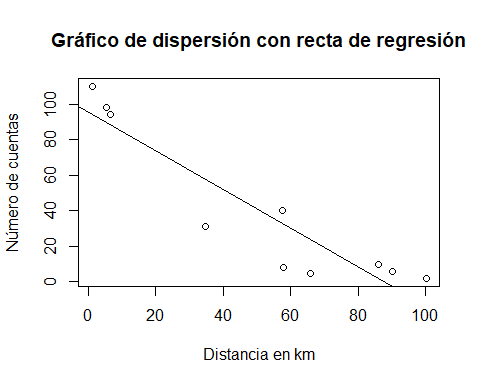
\includegraphics{Practica_6_files/figure-latex/unnamed-chunk-14-1.pdf}

\hypertarget{ejercicio-13-residuos}{%
\subsection{Ejercicio 13: Residuos}\label{ejercicio-13-residuos}}

Llamamos residuos a la diferencia que existe entre los valores del eje Y
y los que predecimos a través de una recta de regresión. Estos valores
los podemos calcular con la función \texttt{resid}. Los residuos
estandarizados se calculan con el valor de un residuo dividido entre una
estimación de su desviación estándar. Lo podemos hacer de forma
automática con la función \texttt{rstandard}. Por último los residuos
estudentizados se calculan con el valor residual de regresión dividido
por su error estándar ajustado. Lo podemos hacer con la función:
\texttt{rstudent}.

\begin{Shaded}
\begin{Highlighting}[]
\FunctionTok{resid}\NormalTok{(modelo)}
\end{Highlighting}
\end{Shaded}

\begin{verbatim}
##          1          2          3          4          5          6          7 
##  15.824925  15.570779   8.807066   8.500073   7.145471   5.804766 -26.643686 
##          8          9         10 
## -18.830406 -24.419631   8.240642
\end{verbatim}

\begin{Shaded}
\begin{Highlighting}[]
\FunctionTok{rstandard}\NormalTok{(modelo)}
\end{Highlighting}
\end{Shaded}

\begin{verbatim}
##          1          2          3          4          5          6          7 
##  1.0784816  1.0622593  0.5721649  0.5661008  0.4307982  0.3843280 -1.6213545 
##          8          9         10 
## -1.1448722 -1.4726329  0.5266739
\end{verbatim}

\begin{Shaded}
\begin{Highlighting}[]
\FunctionTok{rstudent}\NormalTok{(modelo)}
\end{Highlighting}
\end{Shaded}

\begin{verbatim}
##          1          2          3          4          5          6          7 
##  1.0912716  1.0721374  0.5465101  0.5404749  0.4077319  0.3628715 -1.8509341 
##          8          9         10 
## -1.1711614 -1.6134626  0.5014281
\end{verbatim}

\hypertarget{ejercicio-14-predecir-a-travuxe9s-del-modelo-de-regresiuxf3n-un-valor-de-x}{%
\subsection{Ejercicio 14: Predecir a través del modelo de regresión un
valor de
X}\label{ejercicio-14-predecir-a-travuxe9s-del-modelo-de-regresiuxf3n-un-valor-de-x}}

Para ello sustituimos el valor de x que queremos calcular en nuestra
recta de regresión:

\begin{Shaded}
\begin{Highlighting}[]
\NormalTok{y\_6}\FloatTok{.6} \OtherTok{\textless{}{-}} \FloatTok{95.36} \SpecialCharTok{{-}} \FloatTok{1.082} \SpecialCharTok{*} \FloatTok{6.6}
\NormalTok{y\_6}\FloatTok{.6}
\end{Highlighting}
\end{Shaded}

\begin{verbatim}
## [1] 88.2188
\end{verbatim}

\hypertarget{ejercicio-15-generar-dos-conjuntos-de-datos}{%
\subsection{Ejercicio 15: Generar dos conjuntos de
datos:}\label{ejercicio-15-generar-dos-conjuntos-de-datos}}

Queremos generar dos conjuntos de datos, uno para entrenar y crear una
recta de regresión y otro para comprobar la validez de esta.

\begin{Shaded}
\begin{Highlighting}[]
\FunctionTok{library}\NormalTok{(dplyr)}
\end{Highlighting}
\end{Shaded}

\begin{verbatim}
## 
## Attaching package: 'dplyr'
\end{verbatim}

\begin{verbatim}
## The following object is masked from 'package:kableExtra':
## 
##     group_rows
\end{verbatim}

\begin{verbatim}
## The following object is masked from 'package:MASS':
## 
##     select
\end{verbatim}

\begin{verbatim}
## The following objects are masked from 'package:stats':
## 
##     filter, lag
\end{verbatim}

\begin{verbatim}
## The following objects are masked from 'package:base':
## 
##     intersect, setdiff, setequal, union
\end{verbatim}

\begin{Shaded}
\begin{Highlighting}[]
\NormalTok{data }\OtherTok{\textless{}{-}} \FunctionTok{data.frame}\NormalTok{(x\_distancias, y\_cuentas)}
\NormalTok{train }\OtherTok{\textless{}{-}}\NormalTok{ data }\SpecialCharTok{\%\textgreater{}\%}\NormalTok{ dplyr}\SpecialCharTok{::}\FunctionTok{sample\_frac}\NormalTok{(.}\DecValTok{8}\NormalTok{)}
\NormalTok{test }\OtherTok{\textless{}{-}}\NormalTok{ dplyr}\SpecialCharTok{::}\FunctionTok{anti\_join}\NormalTok{(data, train)}
\end{Highlighting}
\end{Shaded}

\begin{verbatim}
## Joining with `by = join_by(x_distancias, y_cuentas)`
\end{verbatim}

\begin{Shaded}
\begin{Highlighting}[]
\NormalTok{train}
\end{Highlighting}
\end{Shaded}

\begin{verbatim}
##   x_distancias y_cuentas
## 1         57.5        40
## 2          1.1       110
## 3         34.7        31
## 4         86.1        10
## 5         90.3         6
## 6          6.6        94
## 7        100.2         2
## 8         57.9         8
\end{verbatim}

\begin{Shaded}
\begin{Highlighting}[]
\NormalTok{test}
\end{Highlighting}
\end{Shaded}

\begin{verbatim}
##   x_distancias y_cuentas
## 1          5.4        98
## 2         65.8         5
\end{verbatim}

\hypertarget{ejercicio-16-generar-el-modelo-otra-vez}{%
\subsection{Ejercicio 16: Generar el modelo otra
vez}\label{ejercicio-16-generar-el-modelo-otra-vez}}

Para generar el modelo de regresión con los datos de entrenamiento
repetimos todos los pasos que para cuando lo generamos la primera vez
pero ahora con los conjuntos de datos de entrenamiento

\begin{Shaded}
\begin{Highlighting}[]
\NormalTok{modelo\_train }\OtherTok{\textless{}{-}} \FunctionTok{lm}\NormalTok{(x\_distancias }\SpecialCharTok{\textasciitilde{}}\NormalTok{ y\_cuentas, train)}
\FunctionTok{summary}\NormalTok{(modelo\_train)}
\end{Highlighting}
\end{Shaded}

\begin{verbatim}
## 
## Call:
## lm(formula = x_distancias ~ y_cuentas, data = train)
## 
## Residuals:
##     Min      1Q  Median      3Q     Max 
## -25.039  -6.242   5.686   9.348  16.651 
## 
## Coefficients:
##             Estimate Std. Error t value Pr(>|t|)    
## (Intercept)  85.1908     7.9516   10.71  3.9e-05 ***
## y_cuentas    -0.8210     0.1461   -5.62  0.00136 ** 
## ---
## Signif. codes:  0 '***' 0.001 '**' 0.01 '*' 0.05 '.' 0.1 ' ' 1
## 
## Residual standard error: 16.25 on 6 degrees of freedom
## Multiple R-squared:  0.8404, Adjusted R-squared:  0.8138 
## F-statistic: 31.58 on 1 and 6 DF,  p-value: 0.001356
\end{verbatim}

\begin{Shaded}
\begin{Highlighting}[]
\FunctionTok{plot}\NormalTok{(train)}
\FunctionTok{abline}\NormalTok{(modelo\_train)}
\end{Highlighting}
\end{Shaded}

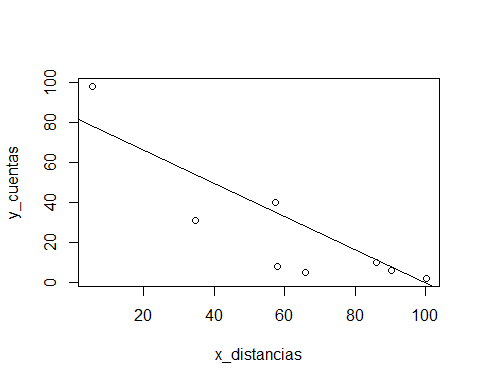
\includegraphics{Practica_6_files/figure-latex/unnamed-chunk-18-1.pdf}

\hypertarget{ejercicio-17-asteriscos-y-r2}{%
\subsection{Ejercicio 17: Asteriscos y
R\^{}2}\label{ejercicio-17-asteriscos-y-r2}}

Los asteriscos que aparecen en la columna de la derecha de los datos
obtenidos con la función \texttt{summary} de nuestro modelo, nos
informan sobre la fiabilidad de nuestro modelo. A más asteriscos menor
es la posibilidad de que la relación que hemos generado entre las
variables se deba al azar. R\^{}2 nos informa sobre la relación
porcentual que existe entre los datos y la línea de regresión que hemos
creado. A más se acerque R\^{}2 al 1 más se acercan los datos de la
variable dependiente a nuestra línea de regresión.

\hypertarget{ejercicio-18-grados-de-libertad}{%
\subsection{Ejercicio 18: Grados de
libertad}\label{ejercicio-18-grados-de-libertad}}

Los grados de libertad del modelo son la cantidad de datos que se
utilizan para estimar los parámetros de un modelo concreto. En el caso
de los modelos de regresión lineal como el que hemos creado, los
parámetros a estimar son la pendiente y la intersección con el eje Y.
Los grados de libertad del modelo se calculan restando el número de
parámetros a estimar a las observaciones del modelo. En nuestro caso
tenemos dos parámetros a estimar y varias observaciones. Si usamos el
primer modelo que hemos creado, sería 10 el número de observaciones
menos 2, el número de parámetros a estimar, lo cual nos daría 8. Si
cogemos el segundo modelo creado (entrenamiento), el resultado sería de
6 porque el número de observaciones es menor. El grado de libertad de un
modelo es relevante porque nos informa sobre la fiabilidad del modelo. A
mayor grado de libertad, más fiable será el modelo, porque tenemos más
observaciones. Siendo este el caso, nuestro modelo original sería más
fiable siguiendo este pensamiento; pero ya que hemos incluido todos
nuestros datos para crearlo, no tendríamos oportunidad de comprobar su
fiabilidad con otro conjunto de datos mediante un método de validación.

\hypertarget{ejercicio-19-varianza}{%
\subsection{Ejercicio 19: Varianza}\label{ejercicio-19-varianza}}

La varianza de un modelo nos informa sobre cómo de correcto es el ajuste
que se ha producido entre la variable dependiente y la independiente, y
con ello comprobar la significancia estadística de nuestra variable
dependiente. En un modelo de regresión lineal, la varianza total de la
variable dependiente (y) se puede descomponer en dos componentes: la
varianza explicada por el modelo (también conocida como suma de
cuadrados de regresión) y la varianza no explicada por el modelo
(también conocida como suma de cuadrados de residuos). Para poder usar
el código posterior es necesario que nuestros valores estén almacenados
en un dataframe; para ello:

\begin{Shaded}
\begin{Highlighting}[]
\NormalTok{train\_df }\OtherTok{\textless{}{-}} \FunctionTok{data.frame}\NormalTok{(train)}
\NormalTok{train\_df}
\end{Highlighting}
\end{Shaded}

\begin{verbatim}
##   x_distancias y_cuentas
## 1         57.5        40
## 2          1.1       110
## 3         34.7        31
## 4         86.1        10
## 5         90.3         6
## 6          6.6        94
## 7        100.2         2
## 8         57.9         8
\end{verbatim}

\begin{Shaded}
\begin{Highlighting}[]
\FunctionTok{is.data.frame}\NormalTok{(train\_df)}
\end{Highlighting}
\end{Shaded}

\begin{verbatim}
## [1] TRUE
\end{verbatim}

Sabiendo que nuestros datos sí están almacenados ahora en un dataframe,
podemos utilizar el siguiente código para calcular la varianza de
nuestro modelo:

\begin{Shaded}
\begin{Highlighting}[]
\FunctionTok{anova}\NormalTok{(modelo\_train)}
\end{Highlighting}
\end{Shaded}

\begin{verbatim}
## Analysis of Variance Table
## 
## Response: x_distancias
##           Df Sum Sq Mean Sq F value   Pr(>F)   
## y_cuentas  1 8342.2  8342.2  31.584 0.001356 **
## Residuals  6 1584.8   264.1                    
## ---
## Signif. codes:  0 '***' 0.001 '**' 0.01 '*' 0.05 '.' 0.1 ' ' 1
\end{verbatim}

\begin{Shaded}
\begin{Highlighting}[]
\NormalTok{var\_total }\OtherTok{\textless{}{-}} \FunctionTok{var}\NormalTok{(train\_df}\SpecialCharTok{$}\NormalTok{y)}
\NormalTok{var\_total}
\end{Highlighting}
\end{Shaded}

\begin{verbatim}
## [1] 1767.982
\end{verbatim}

\begin{Shaded}
\begin{Highlighting}[]
\NormalTok{var\_explicada }\OtherTok{\textless{}{-}} \FunctionTok{sum}\NormalTok{((modelo\_train}\SpecialCharTok{$}\NormalTok{fitted.values }\SpecialCharTok{{-}} \FunctionTok{mean}\NormalTok{(train\_df}\SpecialCharTok{$}\NormalTok{y))}\SpecialCharTok{\^{}}\DecValTok{2}\NormalTok{)}
\NormalTok{var\_explicada}
\end{Highlighting}
\end{Shaded}

\begin{verbatim}
## [1] 10566.63
\end{verbatim}

\begin{Shaded}
\begin{Highlighting}[]
\NormalTok{var\_no\_explicada }\OtherTok{\textless{}{-}} \FunctionTok{sum}\NormalTok{((train\_df}\SpecialCharTok{$}\NormalTok{y }\SpecialCharTok{{-}}\NormalTok{ modelo\_train}\SpecialCharTok{$}\NormalTok{fitted.values)}\SpecialCharTok{\^{}}\DecValTok{2}\NormalTok{)}
\NormalTok{var\_no\_explicada}
\end{Highlighting}
\end{Shaded}

\begin{verbatim}
## [1] 43264.11
\end{verbatim}

Una varianza explicada alta en el modelo significa que las correlaciones
establecidas por el modelo tienen una gran significancia estadística,
mientras que una varianza no explicada alta significaría que el modelo
no está correctamente ajustada, explicada o que hay datos que no cuadran
con las predicciones del modelo. Como en nuestro caso tenemos una
varianza explicada baja en comparación con la varianza no explicada, no
podemos asumir que nuestro modelo sea bueno para realizar predicciones.

\hypertarget{ejercicio-20-validaciuxf3n-del-modelo}{%
\subsection{Ejercicio 20: Validación del
modelo}\label{ejercicio-20-validaciuxf3n-del-modelo}}

El error cuadrático medio es una métrica utilizada para evaluar el
rendimiento de un modelo de regresión lineal mediante una operación de
validación cruzada. Representa la media de los errores cuadráticos entre
las predicciones del modelo y los valores reales en los datos de prueba.
Un valor más bajo indica que el modelo es mejor para ajustarse a los
datos. Podemos calcularlo con el siguiente código:

\begin{Shaded}
\begin{Highlighting}[]
\NormalTok{predicciones }\OtherTok{\textless{}{-}} \FunctionTok{predict}\NormalTok{(modelo\_train, }\AttributeTok{newdata =}\NormalTok{ test)}
\NormalTok{predicciones}
\end{Highlighting}
\end{Shaded}

\begin{verbatim}
##         1         2 
##  4.731117 81.085670
\end{verbatim}

\begin{Shaded}
\begin{Highlighting}[]
\NormalTok{error\_cuadratico\_medio }\OtherTok{\textless{}{-}} \FunctionTok{sqrt}\NormalTok{(}\FunctionTok{mean}\NormalTok{((test}\SpecialCharTok{$}\NormalTok{y }\SpecialCharTok{{-}}\NormalTok{ predicciones)}\SpecialCharTok{\^{}}\DecValTok{2}\NormalTok{))}
\NormalTok{error\_cuadratico\_medio}
\end{Highlighting}
\end{Shaded}

\begin{verbatim}
## [1] 85.11203
\end{verbatim}

Teniendo en cuenta que el error de nuestro modelo es de más de 32
unidades cuadradas, podemos decir que tiene mucho margen de error, ya
que los datos de nuestra variables no son excesivamente altos, llegando
tan solo algunos a superar las 100 unidades.

\hypertarget{ejercicio-21-valores-influyentes}{%
\subsection{Ejercicio 21: Valores
influyentes}\label{ejercicio-21-valores-influyentes}}

Para comprobar si existen valores influyentes en nuestro modelo podemos
usar el método de Cook, que mide la influencia de una observación en el
ajuste del modelo, eliminando la observación y comparando el ajuste del
modelo con y sin ella. Si el ajuste del modelo cambia
significativamente, entonces la observación se considera influyente.
Para ello corremos el siguiente código:

\begin{Shaded}
\begin{Highlighting}[]
\NormalTok{cooksd }\OtherTok{\textless{}{-}} \FunctionTok{cooks.distance}\NormalTok{(modelo\_train)}
\FunctionTok{plot}\NormalTok{(cooksd, }\AttributeTok{pch =} \DecValTok{20}\NormalTok{, }\AttributeTok{main =} \StringTok{"Distancia de Cook"}\NormalTok{)}
\FunctionTok{abline}\NormalTok{(}\AttributeTok{h =} \DecValTok{3}\SpecialCharTok{/}\FunctionTok{length}\NormalTok{(cooksd), }\AttributeTok{col =} \StringTok{"red"}\NormalTok{)}
\end{Highlighting}
\end{Shaded}

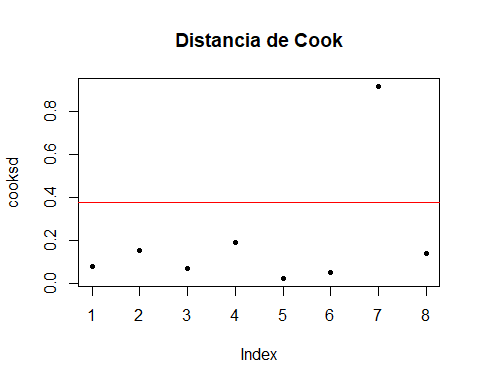
\includegraphics{Practica_6_files/figure-latex/unnamed-chunk-22-1.pdf}
Podemos observar que nuestro valor 7 es un outlier del nuestro modelo, y
por tanto lo podemos considerar como un valor influyente para nuestro
modelo.

\hypertarget{ejercicio-22-supuesto-de-independencia-de-los-residuos}{%
\subsection{Ejercicio 22: Supuesto de independencia de los
residuos}\label{ejercicio-22-supuesto-de-independencia-de-los-residuos}}

El supuesto de independencia de los residuos en un modelo de regresión
lineal es una suposición que hacemos al asumir que los residuos no deben
mostrar patrones o tendencias en su distribución y por tanto que no
están correlacionados entre sí. Si esto no se cumple, no podemos decir
que los errores sean independientes y por ello que las estimaciones que
obtenemos pueden estar sesgadas. Para comprobar dicho supuesto podemos
hacer lo siguiente:

\begin{Shaded}
\begin{Highlighting}[]
\NormalTok{residuos\_train }\OtherTok{\textless{}{-}} \FunctionTok{resid}\NormalTok{(modelo\_train)}
\FunctionTok{plot}\NormalTok{(modelo\_train}\SpecialCharTok{$}\NormalTok{fitted.values, residuos\_train, }\AttributeTok{xlab =} \StringTok{"Valores ajustados"}\NormalTok{, }\AttributeTok{ylab =} \StringTok{"Residuos"}\NormalTok{, }\AttributeTok{main =} \StringTok{"Gráfico de residuos"}\NormalTok{)}
\end{Highlighting}
\end{Shaded}

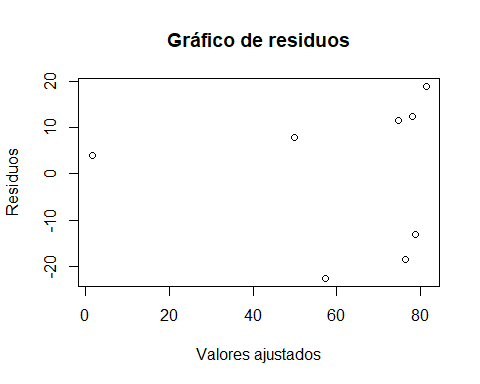
\includegraphics{Practica_6_files/figure-latex/unnamed-chunk-23-1.pdf}
Al graficar los resultados comprobamos que sí existe una tendencia de
agrupación entre los residuos, pero que no todos ellos se encuentran
igualados, teniendo un caso concreto en el que esta tendencia
desaparece. Es muy probable que tengamos que ajustar nuestros datos del
modelo, para generar otro con mejores capacidades predictivas.

\hypertarget{ejercicio-23-comprobar-rango-de-errores}{%
\subsection{Ejercicio 23: Comprobar rango de
errores}\label{ejercicio-23-comprobar-rango-de-errores}}

La primera forma en la que podemos comprobar si el rango de errores para
nuestro modelo es constante sería con la gráfica del anterior ejercicio,
que como hemos hablado tiene un outlier, y por tanto no podemos decir
que permanezcan constantes. Otra forma de hacerlo sería usando el
método/test de Breusch-Pagan:

\begin{Shaded}
\begin{Highlighting}[]
\FunctionTok{library}\NormalTok{(lmtest)}
\end{Highlighting}
\end{Shaded}

\begin{verbatim}
## Loading required package: zoo
\end{verbatim}

\begin{verbatim}
## 
## Attaching package: 'zoo'
\end{verbatim}

\begin{verbatim}
## The following objects are masked from 'package:base':
## 
##     as.Date, as.Date.numeric
\end{verbatim}

\begin{Shaded}
\begin{Highlighting}[]
\NormalTok{bp }\OtherTok{\textless{}{-}} \FunctionTok{bptest}\NormalTok{(modelo\_train)}
\NormalTok{bp}
\end{Highlighting}
\end{Shaded}

\begin{verbatim}
## 
##  studentized Breusch-Pagan test
## 
## data:  modelo_train
## BP = 1.5384, df = 1, p-value = 0.2149
\end{verbatim}

Ya que el p-value que nos ofrece es mayor a nuestro rango de confianza,
no podemos decir que los errores de nuestro modelo permanezcan
constantes, como ya habíamos comprrobado gráficamente. Mediante el uso
de este test el p-value debería permanecer menor a 0'05 en un rango de
confianza del 95\%, para que el supuesto fuese correcto.

\end{document}
